\documentclass[12pt]{article}
\usepackage[utf8]{inputenc}
\RequirePackage[english,spanish,es-tabla]{babel}
\usepackage{multirow}
\usepackage{longtable}
\usepackage{lscape}
\usepackage{fancyhdr}
\RequirePackage{graphicx}
\selectlanguage{spanish}
\RequirePackage{pdfpages}
\usepackage[margin=2cm,headheight=55pt,includeheadfoot]{geometry}
\RequirePackage{multirow}
\RequirePackage{tablefootnote}
\RequirePackage{titlesec}

\titleformat{\section}[block]{\color{black}\Large\bfseries\filcenter}{}{1em}{}
%\titleformat{\subsection}[hang]{\bfseries}{}{1em}{}
\setcounter{secnumdepth}{0}
\pagestyle{fancy}
%definición de las cabezas pares e impares

\fancyhead[LE,LO]{
\includegraphics[width=5cm]{Imagenes/banco-estado-grande.png}}

\fancyhead[RE,RO]{Gerencia de Sistemas \\ Subgerencia de Proyectos}

\title{\textbf{Aspectos Generales}\\\textbf{Proyecto Gobierno de Datos}}

\begin{document}
\vspace*{\fill}
\begin{center}
	{\huge\textbf{Aspectos Generales \\ Proyecto Gobierno de Datos}}
\end{center}

\vspace*{\fill}

\textbf{Mayo 2018}

\newpage
\section{Control de Versiones}
\begin{center}
	\begin{tabular}{|l|l|l|l|}
		\hline
		\textbf{Autor} & \textbf{Fecha} &\textbf{Versión} & \textbf{Descripción}\\
		\hline
		Equipo Desarrollo & 17/05/2018 & 1.0.0 & Creación del Documento\\
		\hline
	\end{tabular}
\end{center}

\newpage
\tableofcontents

\newpage

\section{Introducción}
por desarrollar

\newpage

\section{Tendencia Lenguajes Scala \& Python}
\subsection{Lenguajes de programación más demandados según TIOBE}
\vspace{.04cm}
TIOBE es una empresa con sede en Holanda que, según señala en su página oficial, realiza la comprobación de más de 714 millones de líneas de código de clientes repartidos por todo el globo. Atendiendo a los lenguajes de programación empleados por marcas como Huawei, Bosch o Tomtom, entre muchos otros, TIOBE presenta su lista de lenguajes de programación más populares:

\begin{figure}[!h]
	\begin{center}
		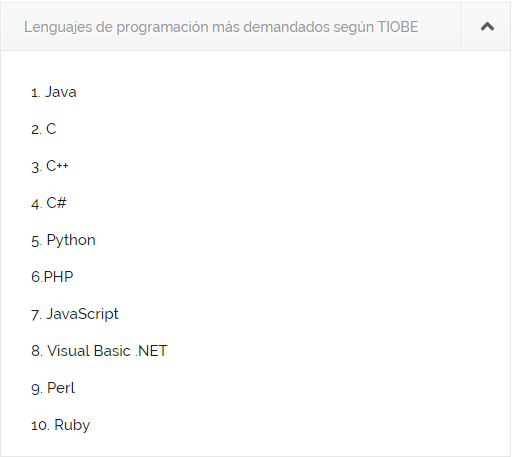
\includegraphics[width=.3\textwidth]{Imagenes/TIOBE.png}
	\end{center}	
\end{figure}

\subsection{Lenguajes de programación más utilizados según GitHub}
La plataforma, una de las más populares para el guardado y revisado de código y en gestión de proyectos y herramientas de software, dispone de una lista de proyectos hospedados. Gracias a ella, la empresa de monitorización de proyectos online Stackify ha podido confeccionar una lista de los lenguajes de programación más populares:

\begin{figure}[!h]
	\centering{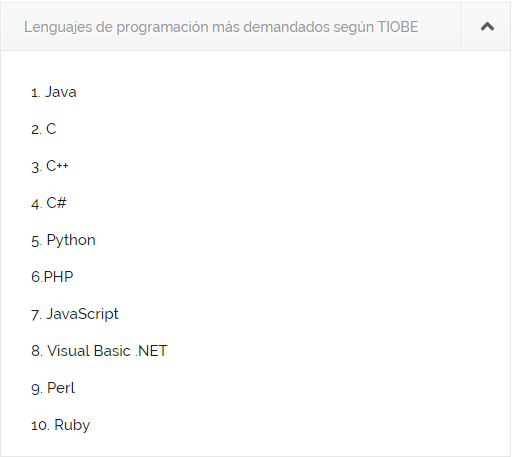
\includegraphics[width=.35\textwidth]{Imagenes/TIOBE.png}}	
\end{figure}

\subsection{Lenguajes de programación más populares según IEEE Spectrum}

Resultados generales de los lenguajes de programación más populares
De las listas anteriores (que representan solo una muestra de las muchas realizadas por muy distintos estudios y empresas de revisión de código) se puede deducir que los lenguajes de programación más demandados en la actualidad son Java, C y Python.

\end{document}
